    \chapter{Methodology}
       \section{SOFTWARE DEVELOPMENT APPROACH}
        Prototyping model is a type of software develpoment model. It is an iterative approach where a basic prototype is constructed to gain a better understanding of the project. This prototype is typically incomplete or lacking many components. The model is then refined based on feedback and system is reconstructed iteratively until desired conditions are met.
         \begin{figure}[hbt!]
            \center{
                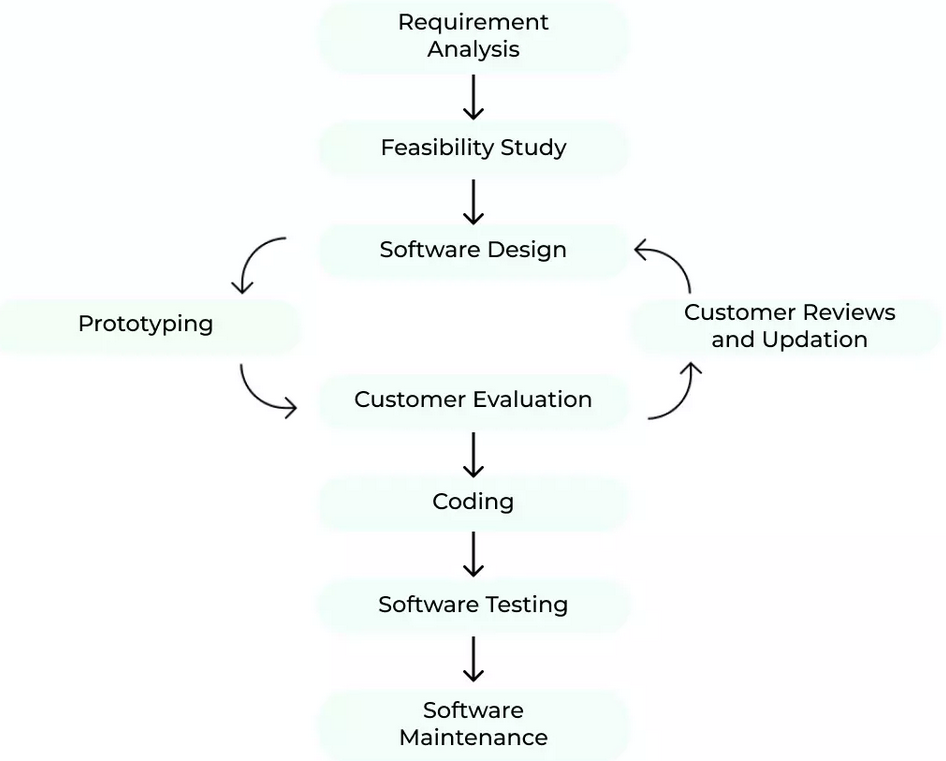
\includegraphics[width=0.75\textwidth]{./img/prototype model.png}
                \caption{Prototype Model for Software Development}
            }
        \end{figure}
        \section{DATA COLLECTION}
        We have decided to use the dataset that consists of 70k REAL faces from the Flickr dataset collected by Nvidia, as well as 70k fake faces sampled from the 1 Million FAKE faces (generated by StyleGAN) that was provided by Bojan which was compiled by xhlulu on kaggle.\\
        \url{https://www.kaggle.com/datasets/xhlulu/140k-real-and-fake-faces}
    
        \section{Implementation}
        Deepfake images are structured and classified into fake and real face images.The images are preprocessed and normalised. The processed image is then fed into a \acrfull*{cnn} model which is repeatedly tested and iterated to generate a model that can predict the deepfake images. The model is tested using test set to generate evaluation metrics.
        \vspace{0.5in}
        \begin{figure}[hbt!]
            \center{
                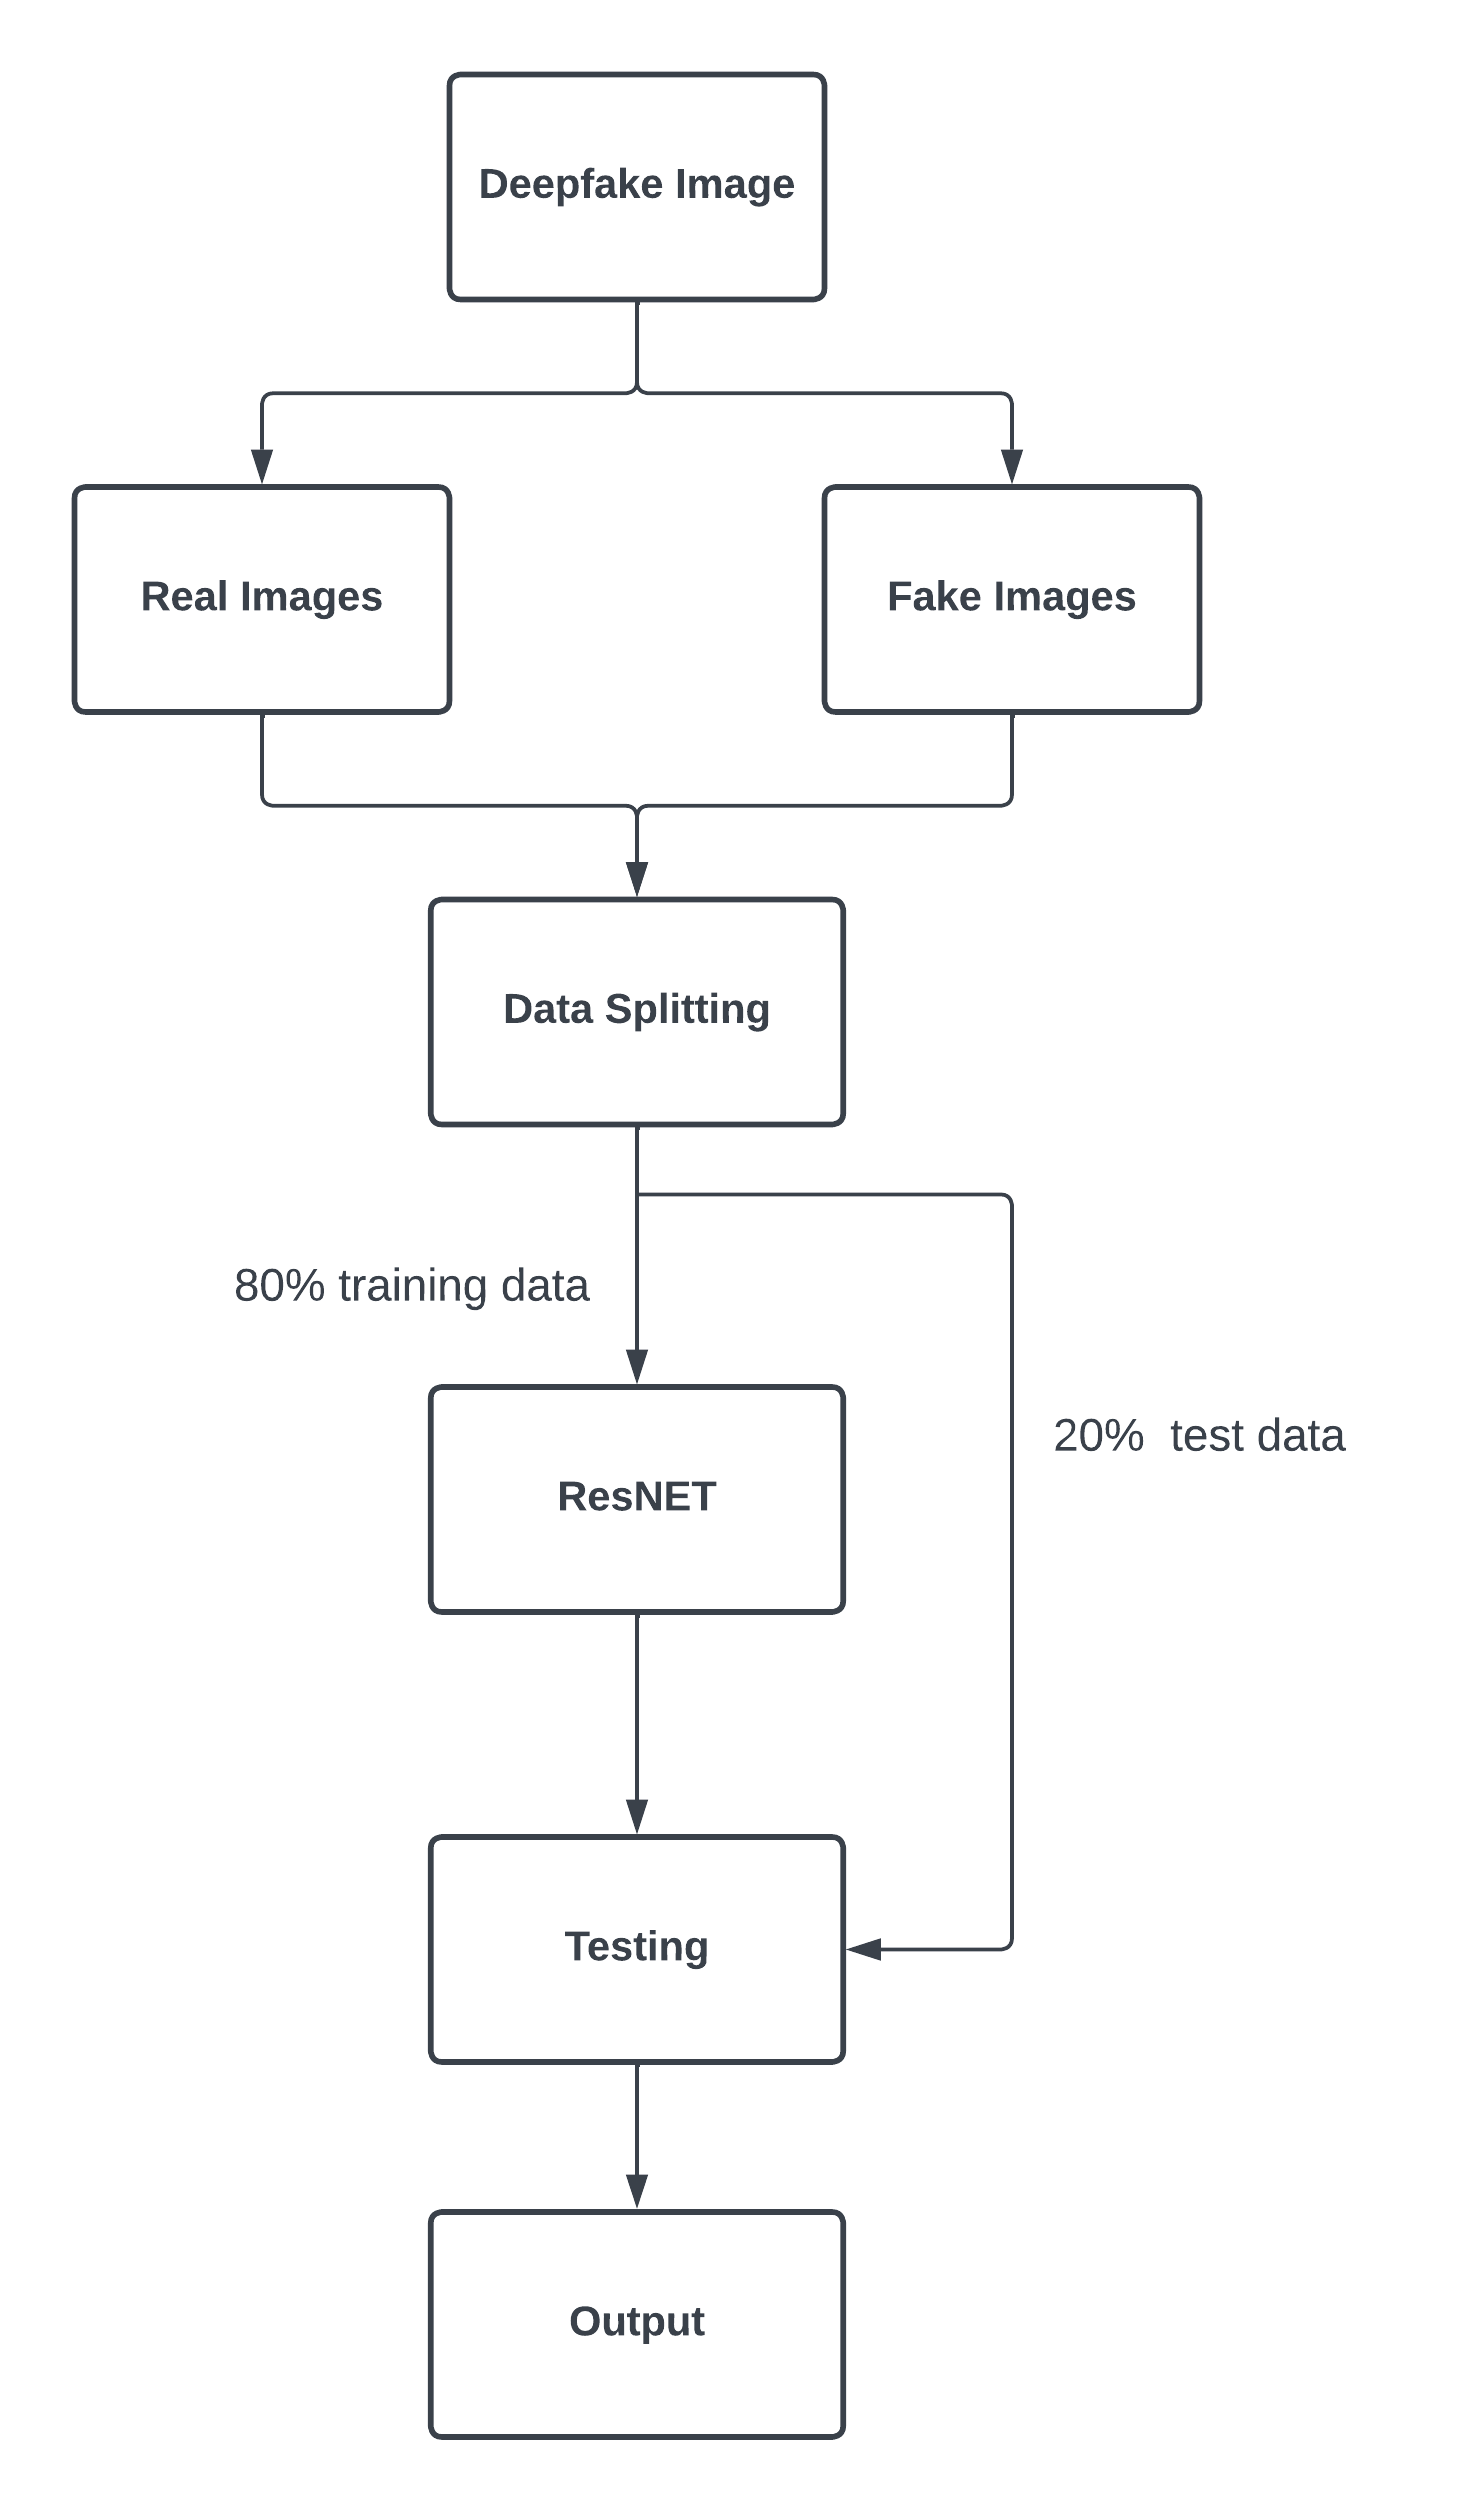
\includegraphics[width=0.25 \textheight]{./img/Block Diagram.png}
                \caption{Block Diagram of Proposed System}
            }
        \end{figure}

        \section{CNN}
        A Convolutional Neural Network (CNN) is a Deep Learning algorithm
        that can take in an input image, assign importance (learnable weights and biases) to various aspects/objects in the image, and be able to differentiate one from the other. The pre-processing required in a CNN is much lower as compared to other classification algorithms. While in primitive methods filters are hand-engineered, with enough training, CNNs have the ability to learn these filters characteristics.The architecture of a CNN is analogous to that of the connectivity pattern of Neurons in the Human Brain and was inspired by the organization of the Visual Cortex. Individual neurons respond to stimuli only in a restricted region of the visual field known as the Receptive Field. A collection of such fields overlap to cover the entire visual area.A CNN typically has three layers: a convolutional layer, a pooling layer, and a fully connected layer.

        Convolutional Neural Networks (CNNs) are utilized for spatial feature extraction . CNNs excel in recognizing patterns within image data by employing
        convolutional layers and filters. The initial layers detect low-level features
        like edges and shapes, while deeper layers abstract higher-level representations of the facial structures. The convolutional process involves
        sliding filters across the input image, enabling the network to identify spatial hierarchies and intricate patterns.
        \begin{figure}[hbt!]
                \center{
                    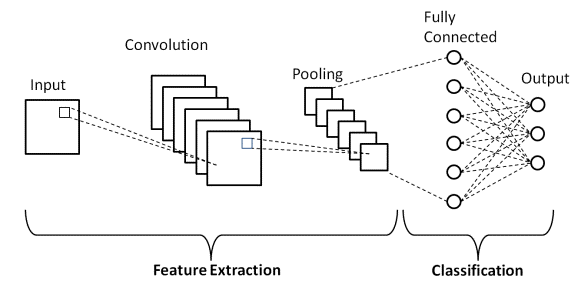
\includegraphics[width=0.9\textwidth]{./img/CNN.png}
                }
                \caption{Convolutional Neural Networks}
        \end{figure}

        \subsection*{ResNet}
        ResNet architecture introduced the concept called Residual Blocks. In this network, we use a technique called skip connections. The skip connection connects activations of a  layer to further layers by skipping some layers in between. This forms a residual block. Resnets are made by stacking these residual blocks together. 
        The approach behind this network is instead of layers learning the underlying mapping, we allow the network to fit the residual mapping. So, instead of say H(x), initial mapping, let the network fit,
        \center{F(x) := H(x) - x 
            which gives H(x) := F(x) + x}

        \begin{figure}[hbt!]
            \center{
                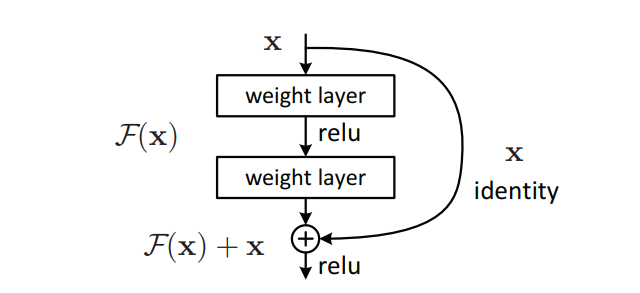
\includegraphics[width=1\textwidth]{./img/ResNet.PNG}
                \caption{ResNet}
            }
        \end{figure}


        \newpage
        \justifying
        \subsection{Gantt Chart}
            \begin{figure}[hbt!]
                \center{
                    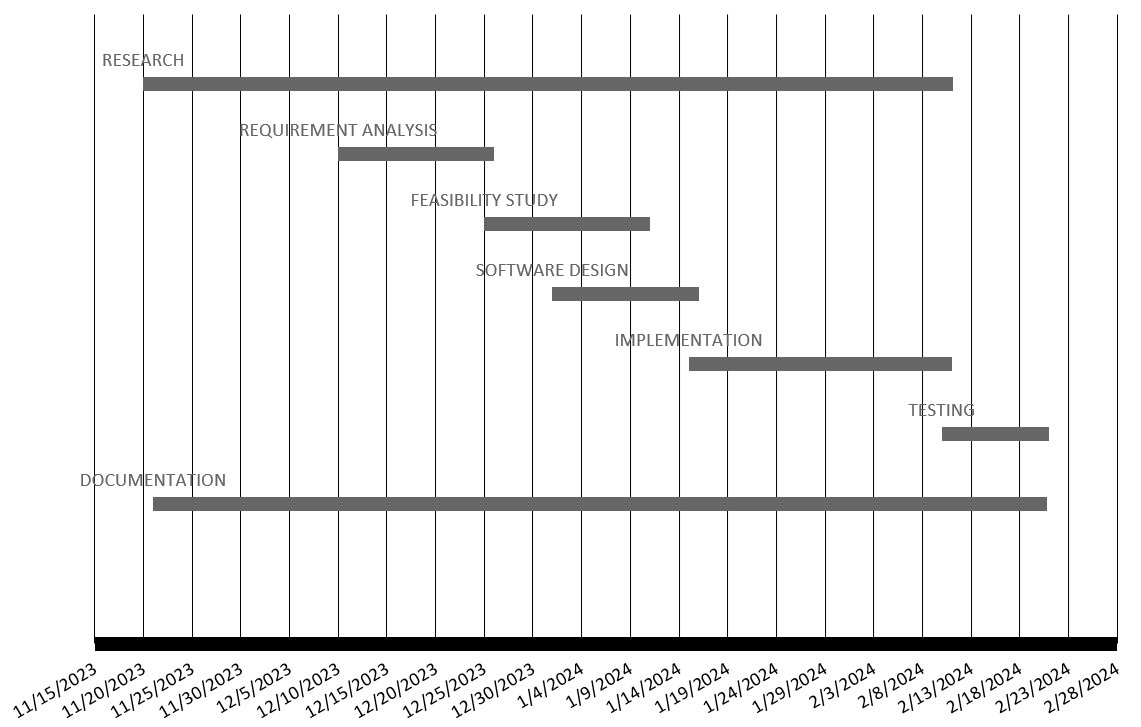
\includegraphics[width=1\textwidth]{./img/GANT_CHART.jpg}
                }
                \caption{Gantt chart}
            \end{figure}

